\section{Provisioning Solutions}

This section describes some of the provisioning solution available today, in particular TOSCA and Open TOSCA, since those are used in the prototypical implementation later on.

\subsection{TOSCA}

\nom{Topology and Orchestration Specification for Cloud Applications}{TOSCA} is a standard that is currently being worked on by the \nom{Organization for the Advancement of Structured Information Standards}{OASIS}\footnote{\url{https://www.oasis-open.org/}}.
Its development is also supported by various industry partners, which include IBM, Cisco, SAP, HP and others.
It's aim is to provide a language that can describe service components and their relations in a cloud environment independent fashion~\autocite{tosca:spec}.

TOSCA defines an XML syntax, which describes services and their relations in a so called service templates.
\autoref{image:tosca:servicetemplate} shows that a service template can be made of up of four distinct parts: Topology templates, orchestration plans, reusable entities, and artifact templates.

\begin{figure}[!htbp]
	\centering
	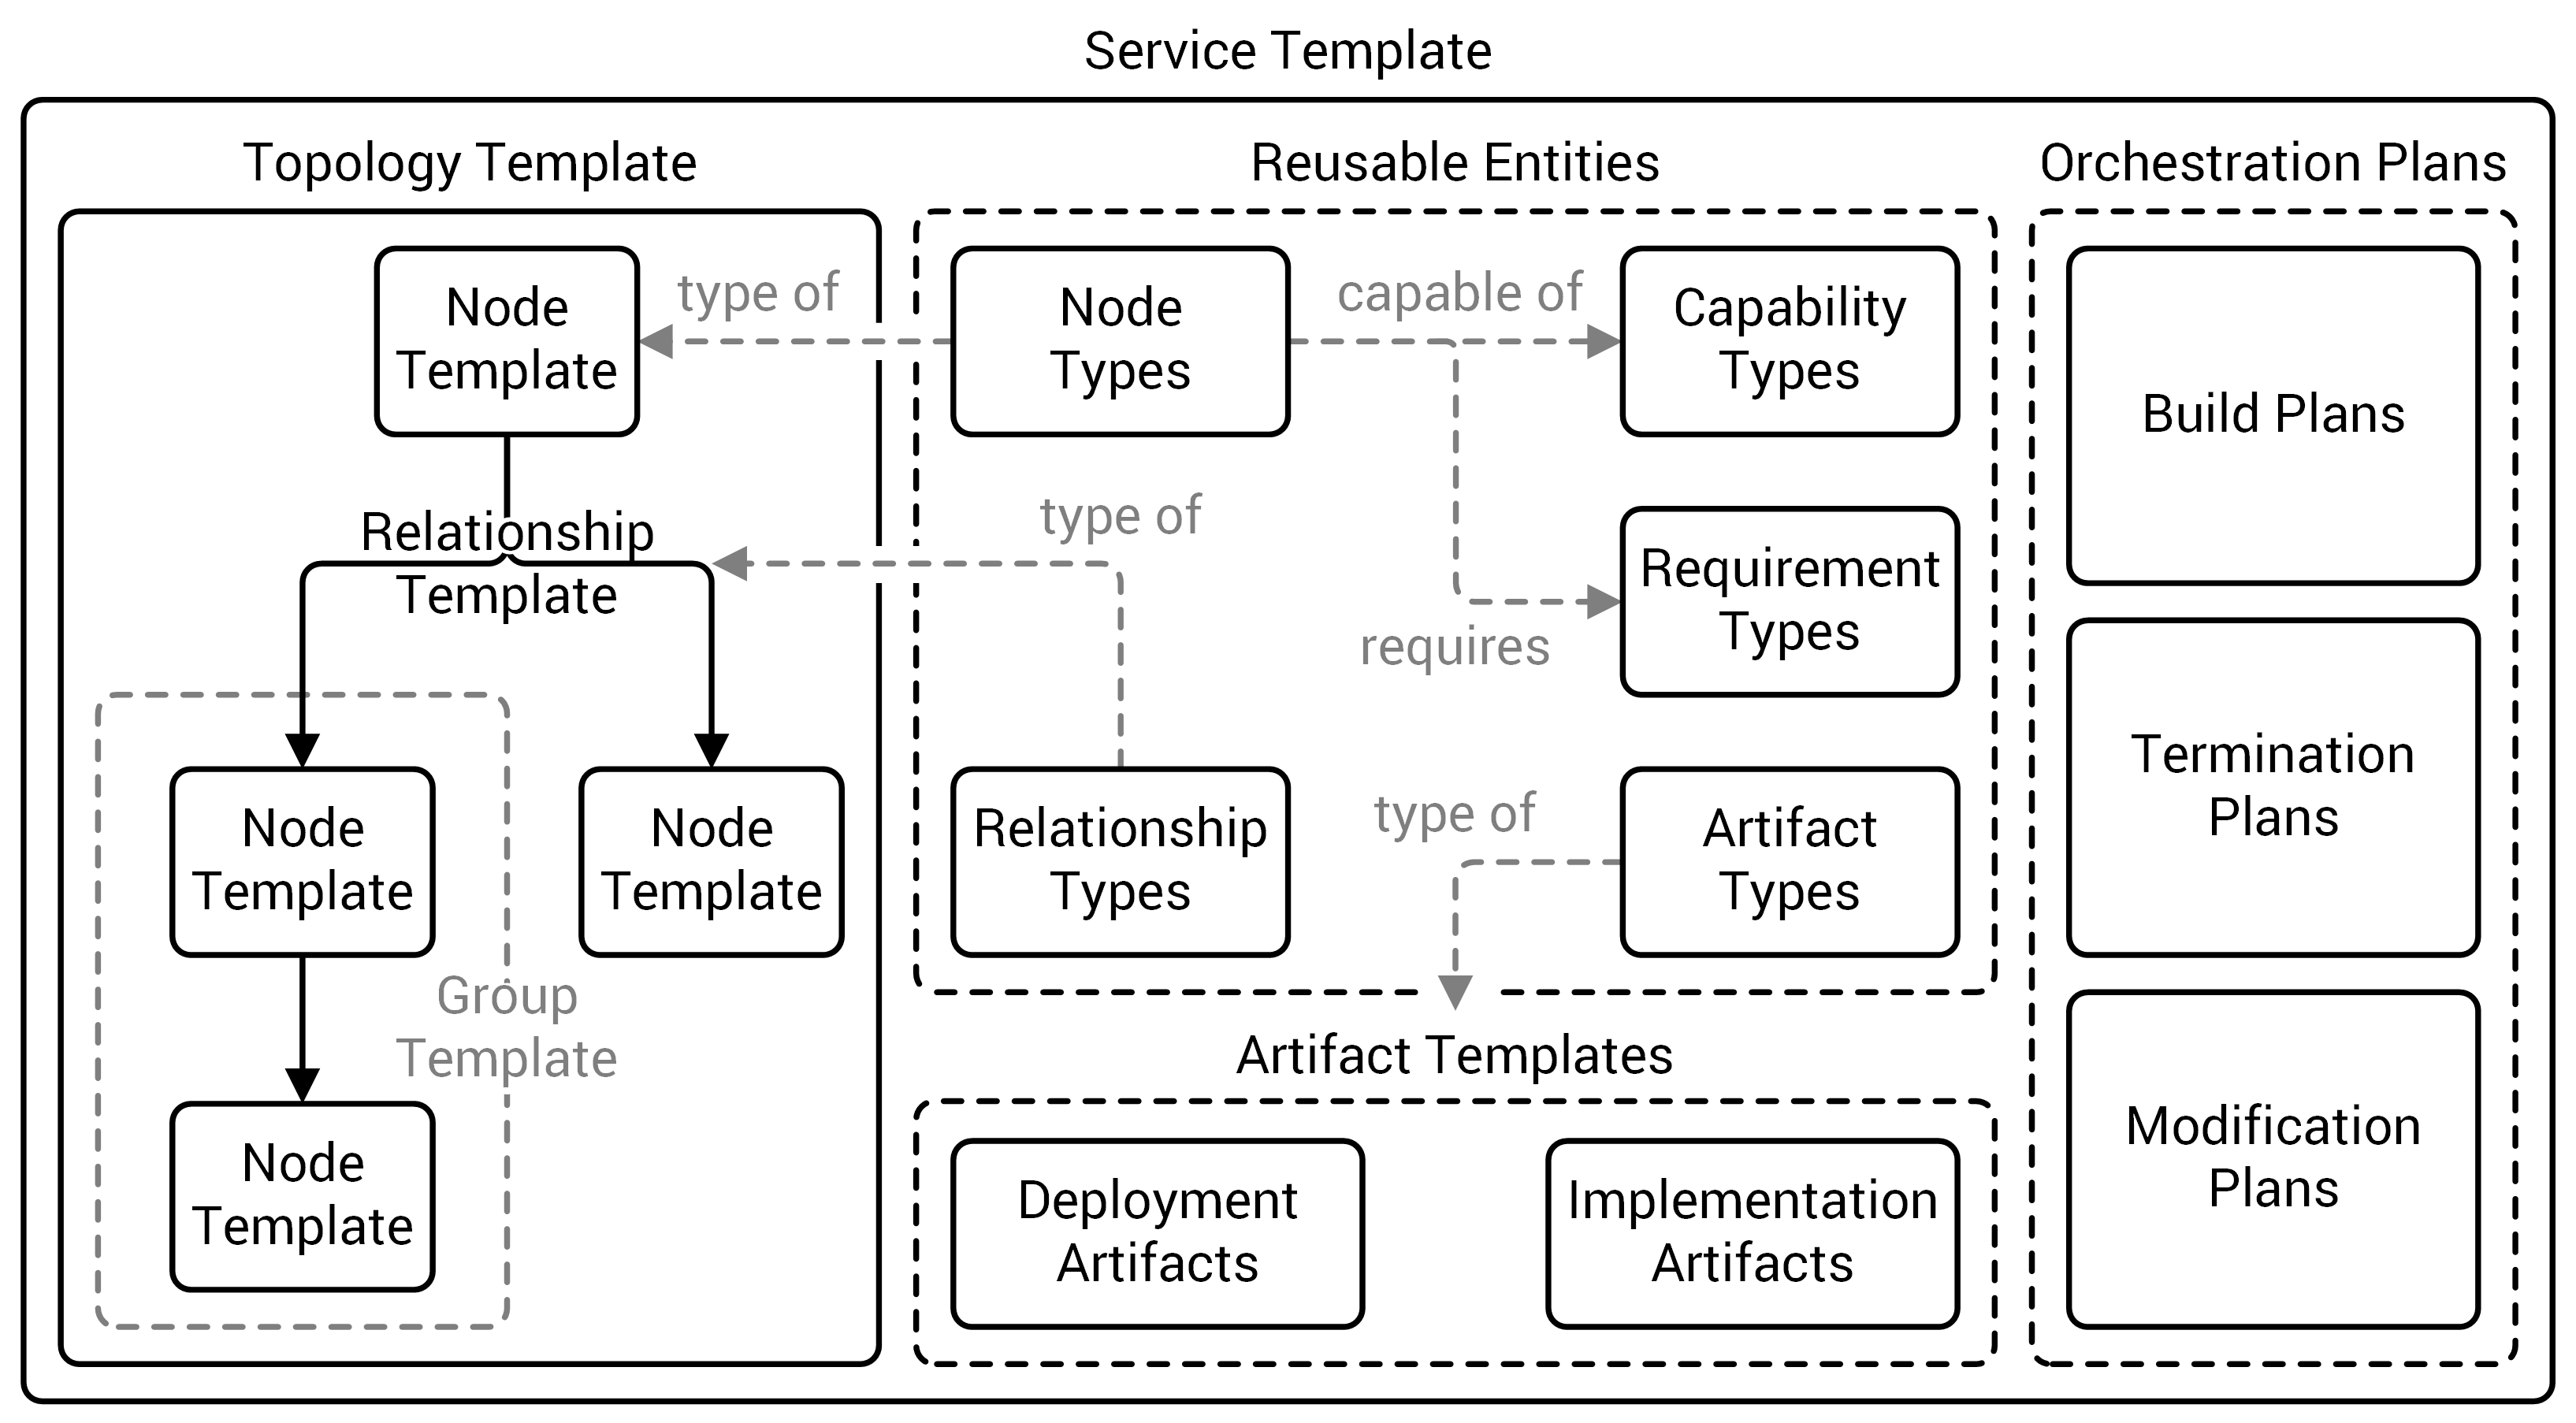
\includegraphics[resolution=600]{fundamentals/assets/service_template}
	\caption{TOSCA service template structure~\autocite[based on][]{tosca:spec}.}
	\label{image:tosca:servicetemplate}
\end{figure}

Topology templates, as seen on the left side of \autoref{image:tosca:servicetemplate}, model the structure of a service as a directed graph.
The vertices of the graph represent nodes, which are occurrences of a specific component, for example, an application server or a database.
These nodes are defined by node types, or by other service templates.
Node types are reusable entities,  as shown in the top center of \autoref{image:tosca:servicetemplate}.
They define the properties of a component, as well as operations to manipulate a component, so called interfaces.
Additionally, node types can be annotated with requirements and capabilities.
These, in turn, are defined by requirement and capability types, which also belong to the group of reusable entities.
This allows for requirement and capability matching between different components.
The edges of the graph represent connections between nodes, which are defined by relationship templates that specify the properties of the relation.
An example for such a connection would be a node A, representing a web service, which is deployed on node B, an application server.
Relationship types are also used to connect requirements and capabilities.

Orchestration plans, shown on the left of \autoref{image:tosca:servicetemplate}, are used to manage the service that is defined by the service template. TOSCA distinguishes between three types of plans: Build plans, termination plans, and modification plans.
Build plans describe, how instances of a service are created.
Termination plans describe, how such a service is removed.
Modification plans manage a service during its runtime.
These plans consist of one or more tasks, i.e., an operation on a node (via an interface) or an external service call, and the order in which these tasks should be performed.
They can be written in \nom{Business Process Model and Notation}{BPMN} or \nom{Business Process Execution Language}{BPEL}, which are already existing languages to describe process models.

The bottom center of \autoref{image:tosca:servicetemplate} shows artifact templates, which represent artifact.
Artifacts are things that can be executed directly (e.g.: scripts, archives) or indirectly (e.g.: URL, ports).
TOSCA further distinguishes between two types of artifacts, namely deployment and implementation artifacts.
Deployment artifacts materialize instances of a node and are used by a build plan to create a service.
An example for this is an \nom{Amazon Machine Images}{AMI}, which creates an Apache server once deployed in a VM.
Implementation artifacts represent the interfaces of components.
Here, an example would be a node that has an interface for starting the particular component described by the node.
This interfaces could be implemented by an implementation artifact like a \textit{.jar} file.

One or more TOSCA service templates are packaged, together with some meta data, into a \nom{Cloud Service Archive}{CSAR}, which is essentially a zip file that contains all files necessary to create and manage a service.
CSAR files can then be executed in a TOSCA runtime environment, also called TOSCA container, to create the service described within.

\subsection{OpenTOSCA}

OpenTOSCA is a browser based open-source implementation of a TOSCA container, created at the IAAS at University Stuttgart, which supports the execution of TOSCA CSAR archives.
\autoref{image:tosca:opentosca} shows the architecture of OpenTOSCA.
Its functionality is realized in three main components, which are the Controller, the Implementation Artifact Engine, and the Plan Engine.
After a CSAR is uploaded to OpenTOSCA it can be deployed in three steps.
In the first step, the CSAR file is unpacked and its content is stored for further use.
The TOSCA XML files are then loaded and processed by the Controller.
The Controller in turn calls the Implementation Artifact Engine and the Plan Engine.
The Implementation Artifact Engine knows how to deploy and store the provided implementation artifacts via plugins.
Plans are then run by the Plan Engine, which also uses plugins to support different plan formats.
OpenTOSCA also offers two APIs, the Container API and the Plan Portability API.
The Container API can be used to access the functionality provided by the container from outside and to provide additional interfaces to the container, like the already existing admin UI, self-service portal, or modeling tool.
The Plan Portability API is used by plans to access topology and instance information~\autocite{opentosca}.

\begin{figure}[!htbp]
	\centering
	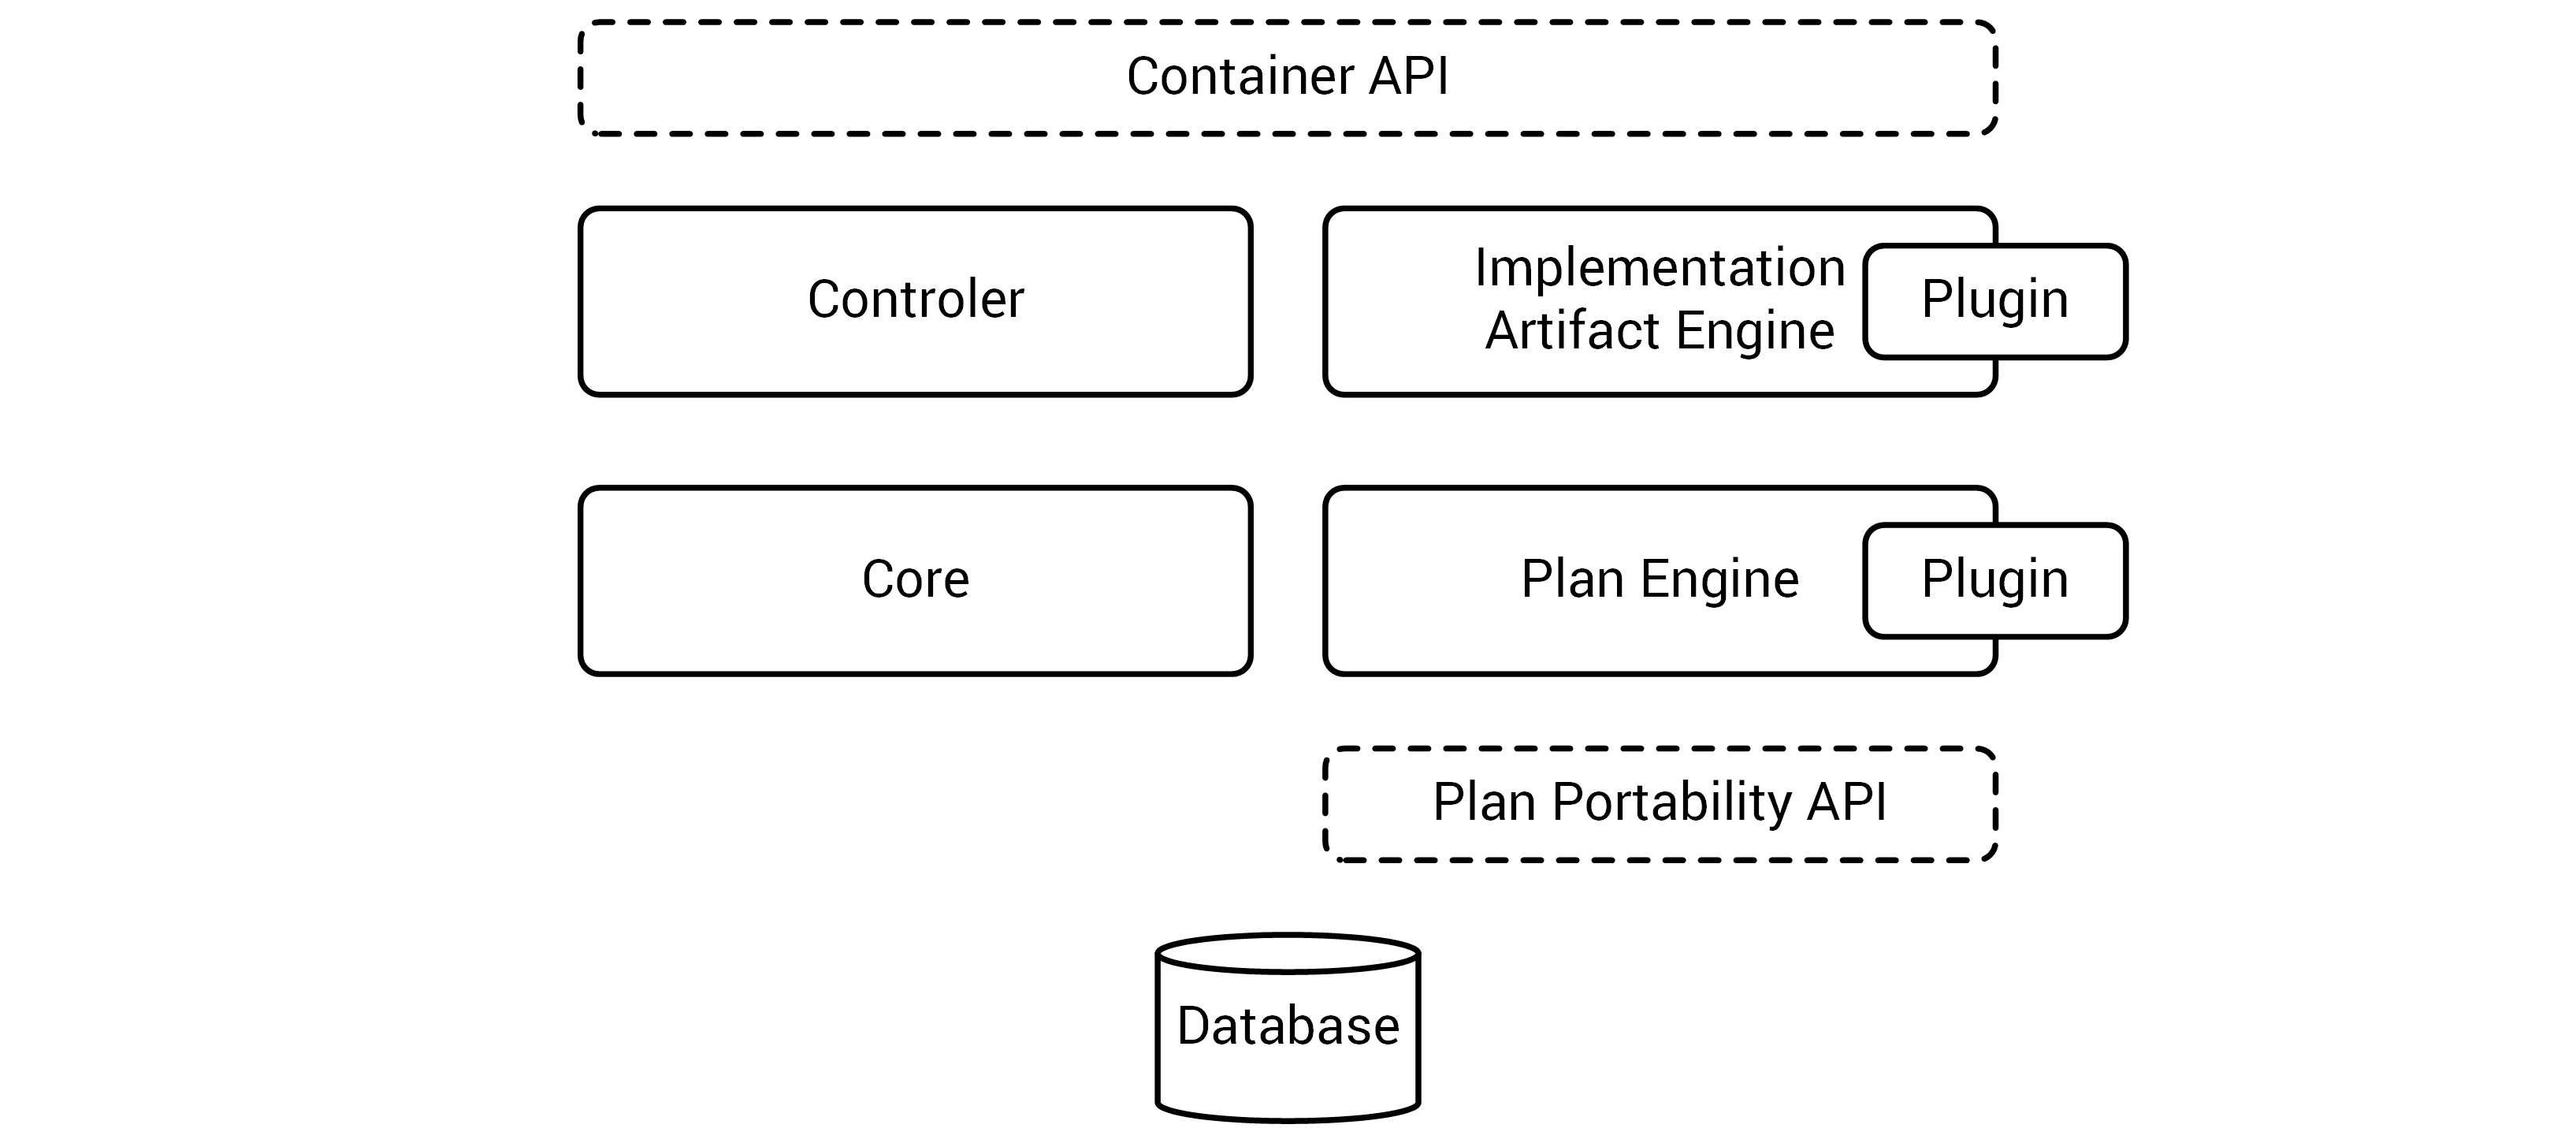
\includegraphics[resolution=600]{fundamentals/assets/opentosca}
	\caption{OpenTOSCA architecture~\autocite[based on][]{opentosca}.}
	\label{image:tosca:opentosca}
\end{figure}
